
\chapter{Implementierung}

In diesem Kapitel wird auf Besonderheiten und Schwierigkeiten bei der Implementierung eingegangen.


%Weitestgehend wie in \autoref{draft:architecture}, aber Futures, tokio, Queues

\section{Continuous Integration mittels Jenkins}

Mittels der Continuous Integration Software Jenkins wird die Rust-Implementation nach jeder Aktualisierung der Quellcode-Repository gebaut.
In einem Jenkinsfile ist hierzu die folgende Pipeline definiert:

\begin{figure}[H]
	\includegraphics[width=\textwidth]{images/jenkins_pipeline_graph.png}
	\caption{Jenkins Pipeline Graph}
	\label{impl:jenkins:pipeline:graph}
\end{figure}

Im folgenden sind die einzelnen Schritte genauer erklärt.


\subsubsection{Schritt \enquote{prepare}}
In diesem Schritt wird überprüft, ob die richtige Version von Rust installiert ist.
Sowohl der Rust Compiler als auch Abhängigkeiten wie Cargo, Clippy oder Tarpaulin werden falls nötig  in diesem Schritt nachinstalliert und aktualisiert.

\subsubsection{Schritt \enquote{check-src}}
Hier wird der Quellcode auf einen schlechtem Programmierstil oder schlechte Programmierpraktiken durch Clippy und auf eine nicht standardkonforme Formatierung überprüft.
Ein erkannter Mangel resultiert in einen Abbruch und einem entsprechendem roten Icon auf der Projektseite auf Jenkins.
Ein Quellcode, der diese Qualitätsstandards nicht erfüllt, wird somit schnellstmöglich abgelehnt.

\subsubsection{Schritt \enquote{Build-Debug}}
In diesem Schritt wird das Projekt im Debug-Modus kompiliert.
In einem Debug-Modus werden nahezu keine Optimierungen durchgeführt, weswegen die Ausführgeschwindigkeit meist mangelhaft ist.
Im falle eines Fehlers in einem Unit-Test, können aus einem Debug-Artefakt jedoch nützlich Informationen gewonnen werden.

\subsubsection{Schritt \enquote{Build-Release-And-Test-Debug}}
Wie der Name bereits vermuten lässt, wird in diesem Schritt das Projekt im Release-Modus übersetzt.
Gleichzeitig wird das zuvor erstellte Debug-Artefakt auf Fehler überprüft, indem Unit-Tests ausgeführt werden.
Ein Release-Artefakt ist stark optimiert und ist für den Produktivbetrieb gedacht.

\subsubsection{Schritt \enquote{Test-Release}}
In diesem Schritt wird das Release-Artefakt mittels Unit-Tests auf Fehler überprüft.
Hierdurch soll sichergestellt werden, dass kein Fehler durch Optimierungen des Compilers aufgedeckt oder verursacht wurde.
Des weiteren soll kein Artefakt archiviert werden, das nicht auf Fehler überprüft wurde.

\subsubsection{Schritt \enquote{Post-Build}}
Dieser Schritt dient zur Zusammenstellung der Testabdeckung der Unit-Tests und der automatisierten  Erstellung der Dokumentation.

\subsubsection{Ergebnis des erfolgreichen Durchlaufs}
Jede Aktualisierung der Quellcoderepository resultiert bei erfolgreicher Kompilation und durchlaufen der Tests in den folgenden Artefakten:
\begin{itemize}
	\item \textbf{Debug-Artefakt}: Kompilation für eine manuelle Fehlersuche mit vielen auf den Quellcode bezogenen Symbolen und ohne Optimierungen durch den Compiler
	\item \textbf{Release-Artefakt}: Kompilat mit Optimierungen für den Produktivbetrieb
	\item \textbf{Testbericht}: Bericht über wie viele Zeilen, Dateien, Klassen und Verzweigungen durch die Unit-Tests getestet wurden.
	\item \textbf{Dokumentation}: Die aus dem Quellcode generierte Dokumentation inklusive der Dokumentationen der Abhängigkeiten.
\end{itemize}

Für jeden erfolgreichen Bauvorgang, werden die erhobenen Informationen in die folgenden Graphen auf der Projektseite auf Jenkins übernommen:

\begin{figure}[H]
	\centering
	\begin{subfigure}{.5\textwidth}
		\includegraphics[width=\textwidth]{images/jenkins_coverage_graph.png}
		\caption{Jenkins Coverage Graph}
		\label{impl:jenkins:coverage:graph}
	\end{subfigure}%
	\begin{subfigure}{.5\textwidth}
		\includegraphics[width=\textwidth]{images/jenkins_warnings_graph.png}
		\caption{Jenkins Warnings Graph}
		\label{impl:jenkins:warnings:graph}
	\end{subfigure}
\end{figure}

\autoref{impl:jenkins:coverage:graph} zeigt die Testabdeckung seit Aufzeichnungsbeginn.
Die frühen und starken Schwankungen resultieren aus Testdurchläufen bei der Einrichtung des Graphen.
\autoref{impl:jenkins:warnings:graph} zeigt Warnungen die der Rust Compiler für die verschiedenen Builds ausgegeben hat.

Die Graphen starten bei unterschiedlichen Versionen, da sie nacheinander eingerichtet wurden.


\clearpage
\section{C++ Algorithmus laden}

Um die optionale Anforderung \reqNumberForLabel{possible:external_algorithm} (siehe \autoref{req:possible:external_algorithm}) umsetzen zu können, muss zuerst die Kommunikation zwischen dem C++ Server und dem Algorithmus analysiert werden:

\begin{figure}[H]
	\begin{tikzpicture}[scale=0.9]
	\begin{umlseqdiag} 
	\umlobject[x=-7,no ddots]{MEC-View-Server}
	\umlobject[x=4,no ddots]{AlgorithmFactory}
%	\umlobject[x=12,class=Algorithm]{a}

	\umlcreatecall[dt=7,class=QueueListener<SensorFrame\_t>,x=-2]{MEC-View-Server}{q}
	\umlcreatecall[dt=5,class=EnvironmentListener,x=2]{MEC-View-Server}{e}
	
	
	\begin{umlcall}[dt=7, op={<<static>> Create(e, q, config\_file)},return=a]{MEC-View-Server}{AlgorithmFactory}
		\umlcreatecall[class=Extension,x=8]{AlgorithmFactory}{a}
	\end{umlcall}
	
	%\begin{umlcall}[op={Start()}]{AlgorithmFactory}{a}
		
	\begin{umlfragment}[type=loop]
	
		\begin{umlcall}[dt=7, type=synchron, op={Add(sensor\_frame)},with return]{MEC-View-Server}{q}
		\end{umlcall}
		
		\begin{umlcall}[dt=18, op={Pop()},return=sensor\_frame]{a}{q}
		\end{umlcall}
		%\begin{umlcall}[dt=7, op={Update(sensor\_frame)}]{a}{a}
		%\end{umlcall}
		\begin{umlcall}[dt=7, op={Update(env\_frame)}]{a}{e}
		\end{umlcall}
		
	\end{umlfragment}
	%\end{umlcall}
	
	\umlsdnode[dt=20]{MEC-View-Server}
	\umlsdnode[dt=13]{q}
	\umlsdnode[dt=4]{e}
	\umlsdnode[dt=29]{AlgorithmFactory}
	\umlsdnode[dt=4]{a}
	
	
	\end{umlseqdiag}
	\end{tikzpicture}
	\centering
	\caption{Instantiierung eines neuen Algorithmus in der C++ Implementation}
	\label{seq_dia:algorithm:cpp}
\end{figure}

In \autoref{seq_dia:algorithm:cpp} ist sowohl die Instantiierung des Algorithmus (Klasse \textit{Extension}) als auch Übermittlung von \textit{SensorFrame}- und \textit{EnvironmentFrame}-Nachrichten (siehe \autoref{msg:sensor_frame} und \autoref{msg:environment_frame}) zu sehen.
Die Kommunikation zwischen dem Algorithmus und der Außenwelt findet über den \textit{QueueListener} und den \textit{EnvironmentListener} statt.
Neue \textit{SensorFrame}-Nachrichten werden in den \textit{QueueListener} eingefügt und zu einem späteren Zeitpunkt asynchron vom Algorithmus ausgelesen.
Eine neue \textit{EnvironmentFrame}-Nachricht übergibt der Algorithmus an den \textit{EnvironmentListener}.
Über diesen wird in der C++ Implementation anschließend die Nachricht an alle Fahrzeuge verteilt.

\todo{?}
Die C++ Implementation reduziert durch dieses Vorgehen die direkte Kommunikation zwischen dem Server und dem konkreten Algorithmus auf den Aufruf von \textit{Create}.
Durch den Austausch dieser Methode kann ein anderer Algorithmus geladen werden.

Damit die Rust-Implementation den C++ Algorithmus Instantiieren kann, muss die Methode \textit{Create} der Klasse \textit{AlgorithmFactory} ordnungsgemäß aufgerufen werden.
Einen gültigen \textit{QueueListener} und \textit{EnvironmentListener} muss zuvor erstellt werden.
Der Fokus liegt somit auf den folgenden Klassen:

\begin{figure}[H]
	\begin{tikzpicture}[scale=0.8, every node/.style={transform shape}]
		\umlclass[x=-11.0,y=-9.5]{mec::algorithm::AlgorithmFactory}{}{
			+ Create(\\
			\quad{}std::weak\_ptr<mec::environment::EnvironmentListener>,\\
			\quad{}std::weak\_ptr<mec::environment::QueueListener<SensorFrame\_t>>,\\
			\quad{}config\_file: std::string\\
			): std::shared\_ptr<mec::extension::Extension>
		}
		
		\umlclass[x=-6.0,y=-5,type=interface]{mec::environment::EnvironmentListener}{}{
			+ Update(frame: std::shared\_ptr<EnvironmentFrame\_t>) \\
			+ Init(init\_message: std::shared\_ptr<InitMessage\_t>) \\
		}
		
		\umlsimpleclass[y=-9.5,type=interface]{mec::extension::Extension}
		
		
		\umlclass[x=-6.0,y=-15,type=interface,template=T]{mec::environment::QueueListener}{}{
			+ Add(sensor\_frame: const std::shared\_ptr<T>): void \\
			+ Pop(): const std::shared\_ptr<T> \\
			+ Pop(timeout: std::chrono::duration<int, std::milli>): const std::shared\_ptr<T> \\
			+ MessageAvailable(): bool \\
			+ GetMessageCount(): int \\
			+ SetStop(stop: bool) \\
		}
		
		\umluniassoc{mec::extension::Extension}{mec::environment::QueueListener}
		\umluniassoc{mec::extension::Extension}{mec::environment::EnvironmentListener}
		\umluniassoc{mec::algorithm::AlgorithmFactory}{mec::extension::Extension}
	\end{tikzpicture}
	\centering
	\caption{Instantiierung eines neuen Algorithmus in der C++ Implementation}
	\label{class_dia:algorithm:cpp}
\end{figure}

Der C++ Algorithmus soll dem Merkmal des Rust Algorithmus entsprechen, um eine Änderung im bestehenden Rust Code möglichst gering zu halten. \todo{liskov}
Eine Änderung im C++ Quellcode ist jedoch untersagt, stattdessen soll weitere Adaptercode die Lücke schließen. \todo{SRP}
In einem ersten Schritt wird der Methodenaufruf von \textit{AlgorithmFactory::Create} in Rust zugänglich gemacht werden.
Anschließend wird der nötige Adaptercode implementiert, um den C++ Algorithmus dem Rust-Merkmal \textit{Algorithm} zu entsprechen.


Aufgrund der wachsenden Komplexität wird auch die Architektur erweitert und aufgeräumt \todo{DIP}.
In \autoref{draft:architecture} ist die erweiterte Version zu sehen.
Es lohnt sich nun, das Projekt in weiteren Crates aufzuteilen.

\begin{figure}[H]
	\centering
	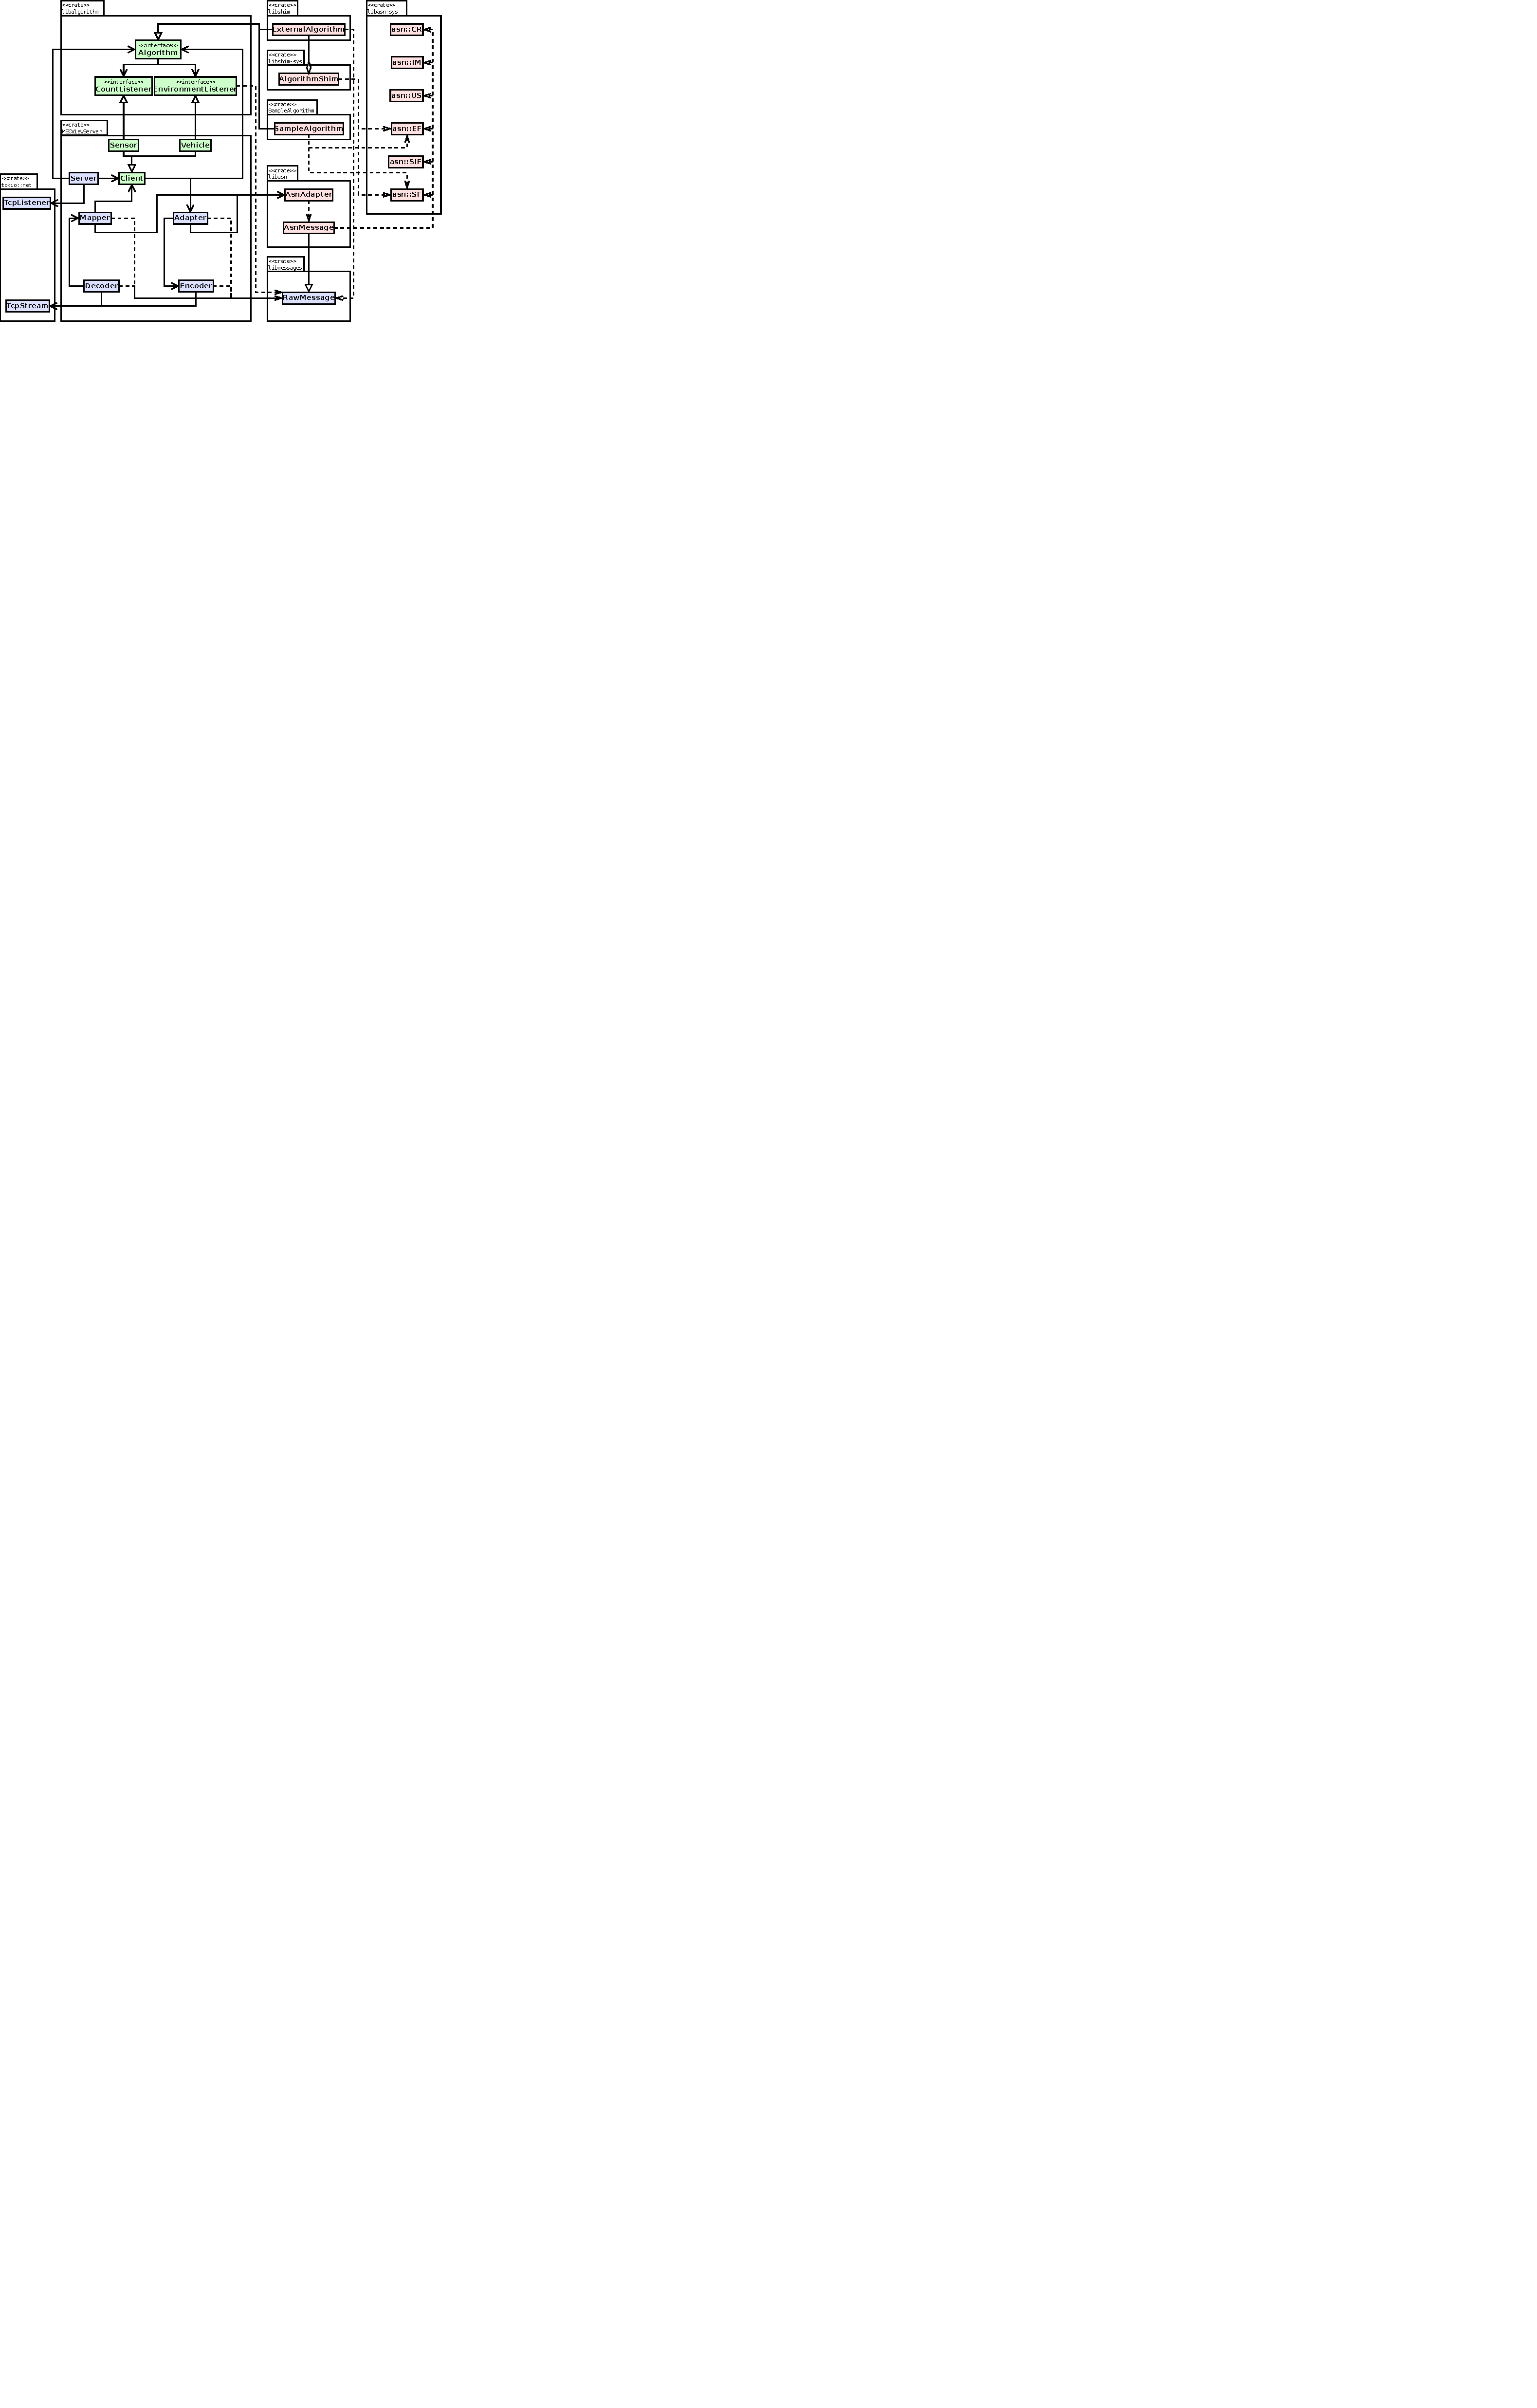
\includegraphics[width=3.3\textwidth]{dia/architecture_v2}
	\caption{Architekturentwurf}
	\label{draft:architecture_v2}
\end{figure}

Die \textit{Alogirhtm}-Schnittstelle und die \textit{RawMessage}-Hilfsklasse wird in jeweils eine eigene Crate verschoben. \todo{DIP}
Die \textit{asn::Message} wird in \textit{AsnMessage} umbenannt und zusammen mit der \textit{AsnAdapter}-Klasse in die neue Crate \textit{libasn} verschoben.
Auch der \textit{SampleAlgorithm} wird in eine extra Crate verschoben.
Zwei weiteren Crates binden den externen C++ Algorithmus ein: \textit{libshim-sys} um den C++ Code in Rust zugänglich zu machen (analog zu \textit{libasn-sys}) und \textit{libshim} für die Implementation der \textit{Algorithm}-Schnittstelle und des Adaptercodes.

Die neuen Abhängigkeiten zwischen den Crates sind in \autoref{draft:architecture_v2_packages} zu sehen und entsprechen nun dem \enquote{Dependency Inversion Principle}.

\begin{figure}[H]
	\centering
	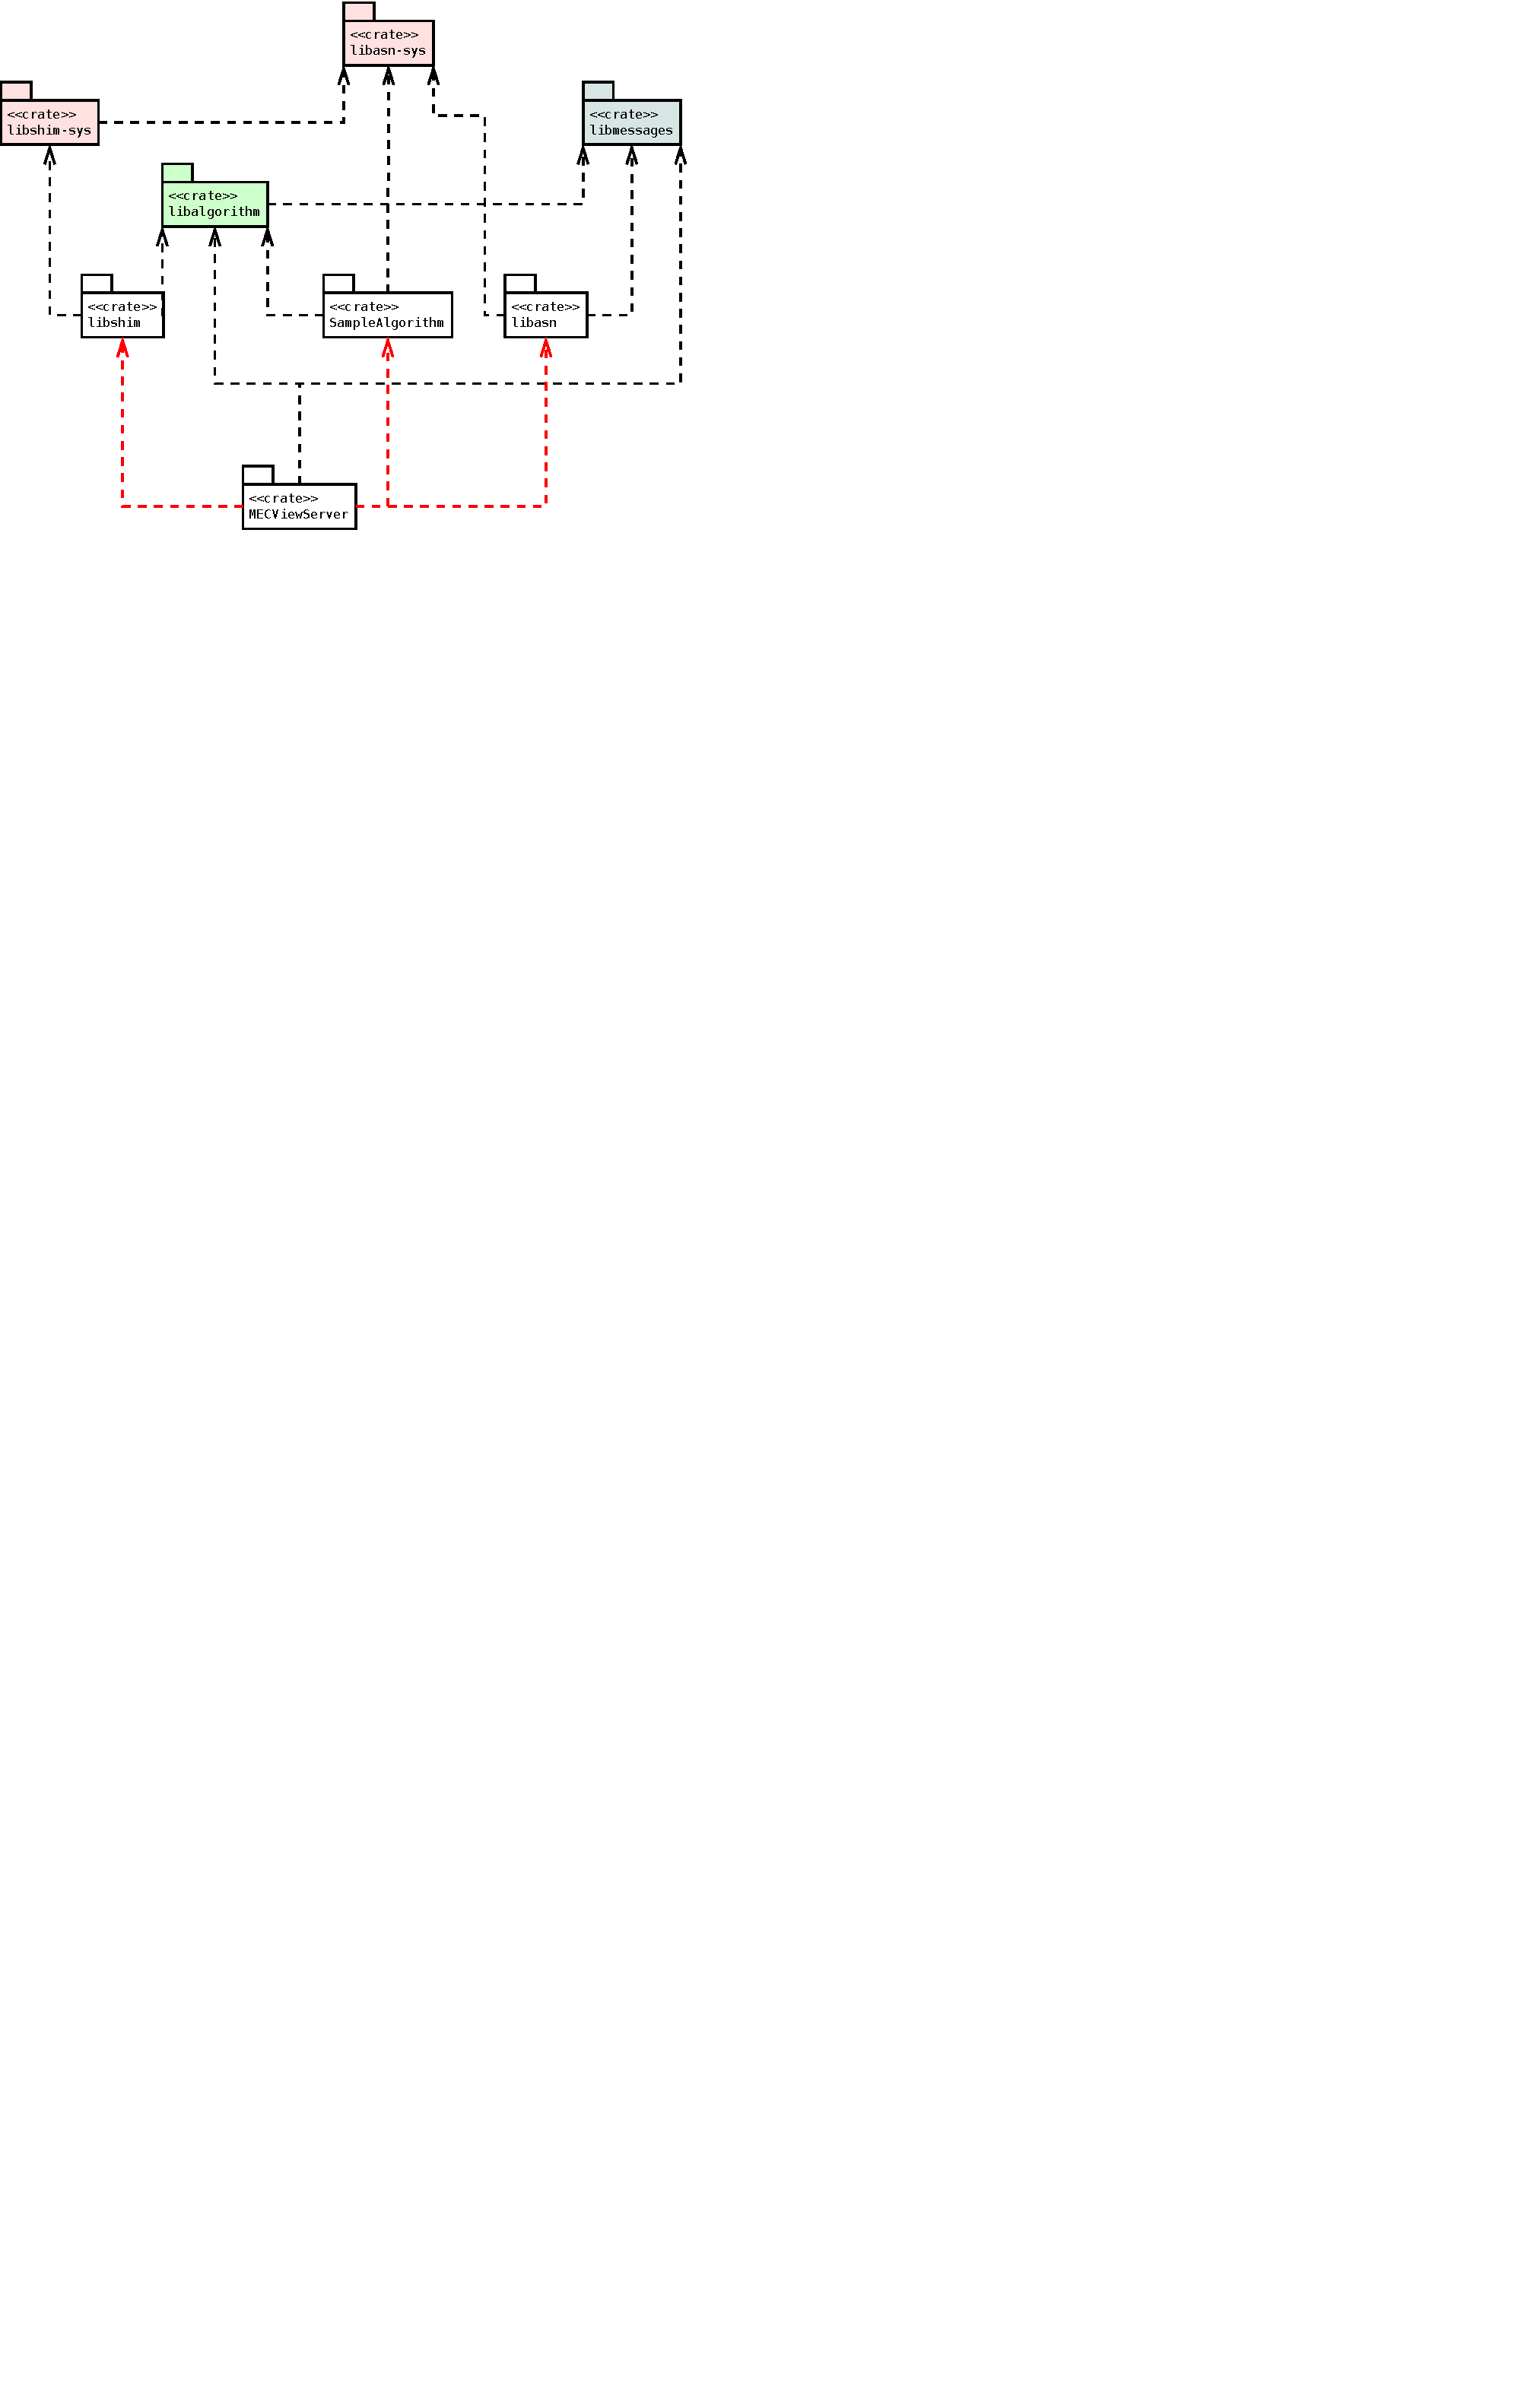
\includegraphics[width=1.9\textwidth]{dia/architecture_v2_packages}
	\caption{Architekturentwurf}
	\label{draft:architecture_v2_packages}
\end{figure}

Die roten Abhängigkeiten entstehen erst durch die Wahl einer Nachrichtentechnologie und des auszuführenden Algorithmus.
\todo{??}
Daher können sie als schwache Abhängigkeiten betrachtet werden.

\todo{schwierig, bindgen nix c++}




\todo{?? updated usecases}

\todo{binary vs source code}

\clearpage
\section{Startparameter}

\todo{show --help}

\helpinclude
	{help}
	{Hilfsinformationen der Rust-Implementation mit allen möglichen Parametern}
	{sections/help.info}

\subsection{?? Unsichtbare Asynchronität des Algorithmus}
\todo{impl Algorithm for Sender<..> proxy communication}

\section{?? Bindgen für ASN}

\label{impl:issue:ffi}
\todo{schnell problem: kein asn->rs compiler, c bindings aufwending -> autogen via bindgen}

\todo{link issues fixed in commit d5d694c}

\todo{impl Drop / free structs, important but do not overengineer}

\section{...}

\todo{bzgl coverage viele tests für encodieren / decodieren, server instanz nicht getestet weil nur mit tokio verdrahtet... schwierig zu testen}


\todo{tdd schwierig weil viel integration mit framework / async, schnell wird daraus integrationstest(?, unerwünscht)}

\todo{rust-clippy: https://github.com/rust-lang-nursery/rust-clippy}


\section{Strategien für Performance}

\todo{\enquote{bypass} via RawMessage for algorithm->many vehicles}





\todo{diagramm: jede future ein eigenes "paket", queues dazwischen für kommunikation}

\todo{catch panic? mention how in \autoref{rust:no_null}}

\todo{SRP, impl Object separat from impl CommandProcessor for Object, testability?}


\section{Schwierigkeit: Heap nicht gleich Heap}

\todo{deadlock im heap allokieren, rust heap muss von rust aufgeräumt werden, libc von libc, asn+c++-alg -> libc}


\subsection{Tokio}

	\subsection{Generalisierung mittels Aufzählung für nicht erweiterbare Anzahl von Elementen}
	
	\subsection{libmessages make unsafe libmessages-sys safe}
	
	\subsection{Vorgehen, bindgen tests, C/unsafe/wrapper -> nach sicher ->  architektur entwickeln}
	

	
	\subsection{Unerwartete Schwierigkeiten}
	
	\todo{Trailing zeroes issue, commit a02496d + tagged, libmessages/src/asn.rs:17 bzw :31 bzw :32 Ok((result.encoded as usize + 7) / 8}
	
	\todo{unterschiedlicher Heap libc / rust --> Rust Heap wird von Rust aufgeräumt, libc von libc... or deadlock}
	
	\todo{jenkins clippy nightly often broken}
	
	\todo{RawMessage<T> machts leben schwer}
	
	
	\subsection{--help}

\todo{bei der entwicklung nie segfault/deadlock gehabt, nur einmal heap problem wegen libc}


\section{Valgrind: Race Conditions all over the place}

\section{Mock TDD}